\documentclass[a4paper,11pt]{article}

\usepackage[utf8]{inputenc}
\usepackage[T1]{fontenc}
\usepackage{lmodern}
\usepackage[margin=22mm]{geometry}
\usepackage{xcolor}
\usepackage{enumitem}
\usepackage{array}
\usepackage{booktabs}
\usepackage{colortbl}
\usepackage{fancyhdr}
\usepackage{titlesec}
\usepackage{hyperref}
\usepackage{tabularx}
\usepackage{ragged2e}
\usepackage{amsmath,amssymb,nicefrac}
\usepackage{xfp}            % arbitrary-precision arithmetic
\usepackage{pgfplots}
\usepackage{pgfplotstable}
\usepackage{caption}
\pgfplotsset{compat=1.18}
\usetikzlibrary{patterns}

% Figures may be compiled from applications/ (their native home on
% DRAFT/006) or from the repo root; try both.
\graphicspath{{./}{./applications/}}

% ── Brand palette ────────────────────────────────────────────────────────
\definecolor{accent}{HTML}{2F6F4E}
\definecolor{accentdark}{HTML}{234F38}
\definecolor{accentlight}{HTML}{EBF3EE}
\definecolor{darktext}{HTML}{1E1E1E}
\definecolor{graytext}{HTML}{646464}
\definecolor{goldcol}{HTML}{D4A017}
\definecolor{btccol}{HTML}{F7931A}
\definecolor{modelcol}{HTML}{4A90D9}
\definecolor{attackcol}{HTML}{C0392B}
\definecolor{lowcol}{HTML}{2E86C1}
\definecolor{highcol}{HTML}{8E44AD}

\hypersetup{colorlinks=true, linkcolor=accentdark, urlcolor=accentdark, citecolor=accentdark}

% ── Headers / footers ────────────────────────────────────────────────────
\pagestyle{fancy}
\fancyhf{}
\renewcommand{\headrulewidth}{0pt}
\fancyhead[R]{\small\textit{\color{graytext}The Security Tax --- Great Wall}}
\fancyfoot[C]{\small\color{graytext}Page \thepage}
\fancypagestyle{plain}{\fancyhf{}\fancyfoot[C]{\small\color{graytext}Page \thepage}}

% ── Section styling ──────────────────────────────────────────────────────
\titleformat{\section}{\Large\bfseries\color{accent}}{}{0em}{}
  [\vspace{-0.6em}{\color{accent}\rule{\textwidth}{0.5pt}}]
\titleformat{\subsection}{\large\bfseries\color{darktext}}{}{0em}{}
\titleformat{\subsubsection}{\normalsize\bfseries\color{darktext}}{}{0em}{}

% ── Table helpers ────────────────────────────────────────────────────────
\newcommand{\theaderrow}{\rowcolor{accent}}
\newcommand{\taltrow}{\rowcolor{accentlight}}

% ══════════════════════════════════════════════════════════════════════════
% LIVE MODEL COMPUTATION (all derived from parameters + data)
% ══════════════════════════════════════════════════════════════════════════
%
% ── Model parameters ─────────────────────────────────────────────────────
%   σ  = severity multiplier (total-loss × uninsured-premium)
%   π_j = jewelry insurance pure premium rate (fraction of value/year)
%   r_j = jewelry-relevant crime rate (burglary per 100K)
%   m   = underreporting multiplier (Lopp: 2-3×)
%
\def\SevMult{6}          % 3× (total vs partial loss) × 2× (uninsured risk premium)
\def\JewPure{0.009}      % 0.9% pure premium rate
\def\JewCrime{229}       % US avg burglary rate per 100K
\def\UnderMult{3}        % baseline underreporting (Lopp estimate)

% ── Transfer coefficient ─────────────────────────────────────────────────
%   κ = σ × π_j / r_j   (cost per unit of per-100K crime rate)
\edef\kappa{\fpeval{\SevMult * \JewPure / \JewCrime}}

% ── Raw data ──────────────────────────────────────────────────────────────
%   Year  Attacks  IndivWhales(K)  BTC_price  Gold_avg
%   Whale estimates: individual holders with >$100K in BTC,
%   excluding institutions, ETFs, exchange company wallets.
%   Includes self-custody AND individual exchange customers.
%
%   2014    1        10      318    1266   (at $318, need 314 BTC)
%   2015    5        15      430    1160
%   2016    4        50      960    1251   (at $960, need 104 BTC)
%   2017   12       500   14156    1257   (bull run, $14K, need 7 BTC)
%   2018   25       200    3693    1269   (crash)
%   2019    8       250    7160    1393
%   2020   14       600   29000    1770   (at $29K, need 3.4 BTC)
%   2021   33      1000   46300    1799   (peak)
%   2022   23       400   16500    1800   (FTX)
%   2023   18       700   42000    1943
%   2024   41       900   93000    2386   (ETFs launched; ETF holders excl)
%   2025   70      1000   88445    3435
%   2026*  28 YTD  1100   97000    ~3500  (103 days; annualized ~99)

% Attacks
\def\aXIV{1}    \def\aXV{5}    \def\aXVI{4}    \def\aXVII{12}
\def\aXVIII{25} \def\aXIX{8}   \def\aXX{14}    \def\aXXI{33}
\def\aXXII{23}  \def\aXXIII{18}\def\aXXIV{41}  \def\aXXV{70}

% 2026 YTD --- pulled from jlopp/physical-bitcoin-attacks on 22 Apr 2026.
% The repo's dated list runs Jan 1 through Apr 13, 2026 (103 elapsed days).
% 2025 is held at its original working-draft value (70); the Lopp repo
% revised downward to 48--56 post-publication, depending on inclusion
% criteria, but this paper's 2019--2025 series is kept intact to preserve
% authorial consistency. The update is confined to the 2026 YTD cells.
\def\aXXVIytd{28}     % documented attacks Jan 1 -- Apr 13, 2026
\def\daysXXVI{103}    % days elapsed in 2026 (through Apr 13)

% Individual whale population (thousands)
\def\wXIV{10}    \def\wXV{15}    \def\wXVI{50}    \def\wXVII{500}
\def\wXVIII{200} \def\wXIX{250}  \def\wXX{600}    \def\wXXI{1000}
\def\wXXII{400}  \def\wXXIII{700}\def\wXXIV{900}  \def\wXXV{1000}
\def\wXXVI{1100}

% ── Per-100K attack rates (adjusted for underreporting) ──────────────────
%   ρ(t) = a(t) × m / (W(t) × 1000) × 100000 = a(t) × m × 100 / W(t)
\edef\rhoXIV{\fpeval{\aXIV * \UnderMult * 100 / \wXIV}}
\edef\rhoXV{\fpeval{\aXV * \UnderMult * 100 / \wXV}}
\edef\rhoXVI{\fpeval{\aXVI * \UnderMult * 100 / \wXVI}}
\edef\rhoXVII{\fpeval{\aXVII * \UnderMult * 100 / \wXVII}}
\edef\rhoXVIII{\fpeval{\aXVIII * \UnderMult * 100 / \wXVIII}}
\edef\rhoXIX{\fpeval{\aXIX * \UnderMult * 100 / \wXIX}}
\edef\rhoXX{\fpeval{\aXX * \UnderMult * 100 / \wXX}}
\edef\rhoXXI{\fpeval{\aXXI * \UnderMult * 100 / \wXXI}}
\edef\rhoXXII{\fpeval{\aXXII * \UnderMult * 100 / \wXXII}}
\edef\rhoXXIII{\fpeval{\aXXIII * \UnderMult * 100 / \wXXIII}}
\edef\rhoXXIV{\fpeval{\aXXIV * \UnderMult * 100 / \wXXIV}}
\edef\rhoXXV{\fpeval{\aXXV * \UnderMult * 100 / \wXXV}}

% 2026 annualized: scale YTD by 365/days
\edef\aXXVIann{\fpeval{\aXXVIytd * 365 / \daysXXVI}}
\edef\rhoXXVI{\fpeval{\aXXVIann * \UnderMult * 100 / \wXXVI}}

% ── Annual security cost c(t) = ρ(t) × κ  [as fraction] ─────────────────
\edef\cXIV{\fpeval{\rhoXIV * \kappa}}
\edef\cXV{\fpeval{\rhoXV * \kappa}}
\edef\cXVI{\fpeval{\rhoXVI * \kappa}}
\edef\cXVII{\fpeval{\rhoXVII * \kappa}}
\edef\cXVIII{\fpeval{\rhoXVIII * \kappa}}
\edef\cXIX{\fpeval{\rhoXIX * \kappa}}
\edef\cXX{\fpeval{\rhoXX * \kappa}}
\edef\cXXI{\fpeval{\rhoXXI * \kappa}}
\edef\cXXII{\fpeval{\rhoXXII * \kappa}}
\edef\cXXIII{\fpeval{\rhoXXIII * \kappa}}
\edef\cXXIV{\fpeval{\rhoXXIV * \kappa}}
\edef\cXXV{\fpeval{\rhoXXV * \kappa}}
\edef\cXXVI{\fpeval{\rhoXXVI * \kappa}}

% ── Growth rates ──────────────────────────────────────────────────────────
%   CAGR of attacks 2019-2026: (aXXVIann/8)^(1/7) - 1
%   CAGR of whale pop 2019-2026: (1100/250)^(1/7) - 1
\edef\gAtk{\fpeval{exp(1/7 * ln(\aXXVIann/\aXIX)) - 1}}
\edef\gWhale{\fpeval{exp(1/7 * ln(\wXXVI/\wXIX)) - 1}}
\edef\gNet{\fpeval{(1 + \gAtk)/(1 + \gWhale) - 1}}

% ── Forward-looking PV of security costs ──────────────────────────────────
%   PV(H) = c_2026 × [(q^H - 1) / (q - 1)]
%   where q = (1 + g_net) / (1 + r)
%
%   At r = 10%:
\edef\qTen{\fpeval{(1 + \gNet) / 1.10}}
\edef\pvFiveTen{\fpeval{\cXXVI * (exp(5*ln(\qTen)) - 1) / (\qTen - 1)}}
\edef\pvTenTen{\fpeval{\cXXVI * (exp(10*ln(\qTen)) - 1) / (\qTen - 1)}}
%   At r = 15%:
\edef\qFif{\fpeval{(1 + \gNet) / 1.15}}
\edef\pvFiveFif{\fpeval{\cXXVI * (exp(5*ln(\qFif)) - 1) / (\qFif - 1)}}
\edef\pvTenFif{\fpeval{\cXXVI * (exp(10*ln(\qFif)) - 1) / (\qFif - 1)}}

% ── Sensitivity: underreporting multiplier variants (2026 annualized) ────
\edef\cCurOneX{\fpeval{\aXXVIann * 1 * 100 / \wXXVI * \kappa}}
\edef\cCurTenX{\fpeval{\aXXVIann * 10 * 100 / \wXXVI * \kappa}}

% ── Valuation parameters ──────────────────────────────────────────────
\def\AvgHoldK{300}        % average individual-whale holdings ($K)

% Whale AUM ($B) --- based on 2026 whale population
\edef\WhaleAUMbn{\fpeval{\wXXVI * \AvgHoldK / 1000}}

% Annual aggregate security tax ($B, 2026 annualised)
\edef\AnnualTAMbn{\fpeval{\cXXVI * \WhaleAUMbn}}

% 10-year aggregate security tax ($B, PV at r = 10%)
\edef\TenYrTAMbn{\fpeval{\pvTenTen * \WhaleAUMbn}}


\begin{document}

% ══════════════════════════════════════════════════════════════════════════
% TITLE
% ══════════════════════════════════════════════════════════════════════════
\thispagestyle{plain}
\begin{center}
{\fontsize{24}{28}\selectfont\bfseries\color{accent}The Security Tax}\\[8pt]
{\large Pricing Bitcoin's Physical Vulnerability\\from Insurance Market Data}\\[14pt]
{\color{accent}\rule{80mm}{0.6pt}}\\[10pt]
{\itshape\color{graytext}The case for Great Wall}\\[4pt]
{\small\color{graytext}Yuri da Silva Villas Boas \textperiodcentered{} April 2026}
\end{center}

\vspace{12pt}

\begin{abstract}
\noindent Physical attacks on Bitcoin holders (``\$5 wrench attacks'') are growing at \fpeval{round(\gAtk * 100, 0)}\% annually, while the individual-whale population grows at only \fpeval{round(\gWhale * 100, 0)}\%. The community's consensus defense --- obscurity --- is both the dominant advice and a structural impediment to adoption. Rather than fitting a discount to Bitcoin price model residuals, this paper estimates the security cost from first principles by cross-referencing wrench attack rates with insurance premiums for comparable portable luxury goods. Restricted to individual (non-institutional) holders with >\$100K in BTC, the severity-adjusted annual security cost reaches \fpeval{round(\cXXVI * 100, 2)}\% of holdings at the 2026 annualised pace --- already inside the gold-storage-fee range. Because Bitcoin's value incorporates speculative expectations and the attack trend is worsening, the forward-looking discount exceeds the current cost: \fpeval{round(\pvFiveTen * 100, 1)}\% over a 5-year horizon and \fpeval{round(\pvTenTen * 100, 1)}\% over 10 years at a 10\% discount rate. Great Wall closes this gap through Tacit Knowledge-Based Authentication (TKBA) --- memory-held entropy encoded onto a user-specific perturbation of the Burning Ship fractal, gated by a calibrated Argon2 derivation, with optional outsourcing of a time-lock puzzle to an anonymous Lightning Network marketplace. The project is entirely free software (MIT or Apache-2.0).
\end{abstract}

% ══════════════════════════════════════════════════════════════════════════
\section{The Trend}
% ══════════════════════════════════════════════════════════════════════════

On 12 February 2026, the account \texttt{@BitcoinNewsCom} posted on X:

\begin{quote}\itshape
\textbf{ATTACKS ON BITCOINERS IN FRANCE ACCELERATING} --- Out of 47 documented attacks against Bitcoin holders in France since 2017, 38 have occurred in just the last 13 months.
\end{quote}

\noindent A prominent community account, \texttt{@BitcoinersHQ}, replied: \textit{``No one needs to know you own Bitcoin.''} The original poster endorsed this as \textit{``Golden advice.''}

This exchange reflects an established consensus across the Bitcoin security community:

\begin{itemize}[nosep,leftmargin=1.5em]
  \item Jameson Lopp (Casa CTO): \textit{``The best things Bitcoiners can do to stay safe is to remain private. Don't go around telling anyone about your Bitcoin holdings.''}\footnote{\url{https://www.theblock.co/post/384018}}
  \item Ledger Academy: \textit{``Never share how much bitcoin you own. Keep a low profile online and offline.''}\footnote{\url{https://www.ledger.com/academy/glossary/wrench-attack}}
  \item ChainSec: \textit{``Hide your crypto stickers. Don't wear crypto merch. Blend in completely.''}\footnote{\url{https://chainsec.io/wrench-attack/}}
\end{itemize}

\noindent The reply by \texttt{@yurivillasboas} to the thread above exposed the structural contradiction:

\begin{quote}\itshape
I'm sorry, but that premise undermines propagation of adoption. Plus, everybody cannot be needles in a haystack. If everyone is needle, there's no hay. \textbf{Maximalism vs Obscurity. Choose one.}
\end{quote}

\noindent The community endorses obscurity \textit{in the same threads} where it documents obscurity's failure. Obscurity \textit{is} the security strategy --- and it imposes a measurable cost. This paper estimates that cost.

\begin{figure}[h]
\centering

\includegraphics[width=0.78\linewidth]{./assets/obscure_bitcoiner_horizontal_short.png}
\caption{The \emph{Maximalism vs.\ Obscurity} dilemma, circulated widely among Bitcoin holders. The contradiction the dilemma dramatises is not incidental: it is the community's current physical-security posture.}
\end{figure}

% ══════════════════════════════════════════════════════════════════════════
\section{An Insurance Framework}
% ══════════════════════════════════════════════════════════════════════════

\subsection{How insurance markets price physical security risk}

Insurance premiums for high-value portable goods --- jewelry, luxury watches, collectible cars --- directly price the cost of physical vulnerability. This market is deep, mature, and empirically well-studied. The table below compiles premium quotes from six independent sources:

\begin{center}
\small
\begin{tabular}{l r l}
\toprule
\textbf{Source / tier} & \textbf{Premium} & \textbf{Notes} \\
& (\% of value/yr) & \\
\midrule
\multicolumn{3}{l}{\textit{Specialty jewelry insurers}} \\
Jewelers Mutual\footnote{Jewelers Mutual Group, \textit{Cost of Jewelry Insurance}, 2025. \url{https://www.jewelersmutual.com/jewelry-insurance-explained/cost}} & 1.0--2.0\% & Dominant US specialty insurer; \\
& & surcharge 25--50\% for items $>\$15$K \\
GEICO / Jewelers Mutual\footnote{GEICO, \textit{Jewelry Insurance Through Jewelers Mutual}, 2025. \url{https://www.geico.com/jewelry-insurance/}} & 1.0--2.0\% & White-label of Jewelers Mutual \\
\midrule
\multicolumn{3}{l}{\textit{General insurers / aggregators}} \\
NerdWallet / III\footnote{NerdWallet, \textit{Jewelry Insurance: How It Works}, 2025; Insurance Information Institute, \textit{Floaters and Endorsements}, 2024.} & 1.0--2.0\% & US national average \\
Bankrate\footnote{Bankrate, \textit{How Much Does Jewelry Insurance Cost?}, 2025. \url{https://www.bankrate.com/insurance/homeowners-insurance/jewelry-insurance-cost/}} & 1.0--2.0\% & Avg.\ \$13--\$20 per \$1K/yr \\
Progressive\footnote{Progressive, \textit{Jewelry Insurance FAQ}, 2025. \url{https://www.progressive.com/answers/jewelry-insurance/}} & 1.0--2.0\% & Via endorsement or standalone \\
\midrule
\multicolumn{3}{l}{\textit{Crime-environment variation}} \\
Low-crime rural (e.g.\ New Hampshire)\footnote{ECI Jewelers, \textit{Guide to Jewelry Insurance Cost}, 2025. Burglary rate $\sim$48/100K (FBI UCR 2024).} & $\sim$1.0\% & Burglary $\sim$48/100K \\
US national average\footnote{FBI, \textit{UCR Summary of Reported Crimes}, 2024. Burglary rate 229/100K.} & 1.5\% & Burglary 229/100K \\
High-crime urban (e.g.\ San Francisco)\textsuperscript{6} & 3.0--3.5\% & Burglary $\sim$500/100K \\
\bottomrule
\end{tabular}
\end{center}

\noindent The convergence across independent sources is striking: every major insurer and aggregator quotes 1--2\% of appraised value at the US national average. The premium varies roughly 3$\times$ across the crime spectrum, reflecting the insurer's actuarial estimate of frequency $\times$ severity. The \textbf{pure premium} (net of administrative loading) is approximately 0.9\% at the US average crime rate. This follows from the industry loss ratio: the inland marine line (parent statutory category for personal articles floaters) reports direct loss ratios of 44--49\%,\footnote{AM Best, \textit{Inland Marine Insurance Market Analysis}, 2024. Loss ratio 44--49\% post-pandemic.} implying a pure premium of $\sim$0.5$\times$ the 1.5\% midpoint gross premium $\approx$ 0.75--0.9\%.

\subsection{What Bitcoin lacks}

No insurance market exists for self-custody Bitcoin. This is not an oversight --- it reflects a fundamental obstacle: a wrench attack can extract the \textit{entire} holdings in a single event with no possibility of recovery, reversal, or tracing. An insurer cannot verify the loss, assess negligence, or recover stolen funds.

The absence of insurance means the holder bears the full actuarial risk \textit{plus} an uninsured risk premium --- the additional discount that risk-averse agents demand when they cannot offload tail risk. Under standard CRRA utility ($\gamma = 2$--$5$), the certainty-equivalent cost of a concentrated, total-loss risk is 1.5--3$\times$ the actuarial expectation.\footnote{Pratt, J.W., ``Risk Aversion in the Small and in the Large,'' \textit{Econometrica} 32(1/2), 1964; Eeckhoudt, Gollier \& Schlesinger, \textit{Economic and Financial Decisions under Risk}, Princeton, 2005, Ch.\ 4--5.}

% ══════════════════════════════════════════════════════════════════════════
\section{Model Construction}
% ══════════════════════════════════════════════════════════════════════════

\subsection{Target population}

Not all Bitcoin holders are plausible wrench attack targets. We restrict the analysis to \textbf{individual (non-institutional) holders with >\$100K in BTC}:

\begin{itemize}[nosep,leftmargin=1.5em]
  \item \textbf{Included:} individuals holding via hardware wallets, software wallets, paper wallets, or personal exchange accounts --- anyone who can be physically coerced into transferring funds.
  \item \textbf{Excluded:} exchange company wallets, Bitcoin ETF custodians (Coinbase Custody, Fidelity), corporate treasuries (MicroStrategy), sovereign funds. These entities have professional security, multi-party authorization, and cannot be compromised by coercing a single individual.
\end{itemize}

\noindent The comparison is individual-to-individual: individual jewelry owners face burglary and robbery; individual Bitcoin whales face wrench attacks. The institutional layer is excluded from both sides.

Whale population estimates are necessarily approximate. They are derived from on-chain address clustering (Glassnode), exchange-reported user demographics, and BTC price (which determines the \$100K threshold in BTC terms). We provide sensitivity analysis in Section~\ref{sec:sensitivity}.

\subsection{The security cost formula}

Let $a(t)$ be the number of documented wrench attacks in year $t$, $W(t)$ the estimated individual whale population (thousands), and $m$ the underreporting multiplier. The \textbf{estimated attack rate per 100K whales} is:

\begin{equation}
  \rho(t) = \frac{a(t) \times m}{W(t) \times 1{,}000} \times 100{,}000 = \frac{100\, m \cdot a(t)}{W(t)}
  \label{eq:rate}
\end{equation}

\noindent This is directly comparable to standard crime rates (burglary per 100K, robbery per 100K) used in insurance pricing.

\medskip
\noindent We translate this crime rate into an insurance-equivalent annual cost using the empirical relationship from jewelry insurance:

\begin{equation}
  \boxed{c(t) = \underbrace{\sigma}_{\text{severity}} \times \underbrace{\frac{\pi_j}{r_j}}_{\text{cost per unit crime}} \times\; \rho(t)}
  \label{eq:cost}
\end{equation}

\noindent where:
\begin{itemize}[nosep,leftmargin=1.5em]
  \item $\pi_j = 0.9\%$ --- jewelry pure premium at US average crime rate
  \item $r_j = 229$ --- US average burglary rate per 100K
  \item $\sigma = 6$ --- severity multiplier (derived below)
\end{itemize}

\noindent The ratio $\pi_j / r_j = \fpeval{round(\JewPure / \JewCrime * 100, 5)}\%$ per unit of crime rate is the \textbf{transfer coefficient}: the insurance market's empirical pricing of one unit of per-100K crime rate for portable luxury goods. Multiplying by $\sigma$ adjusts for the greater severity of Bitcoin attacks relative to jewelry theft.

\subsection{Severity multiplier}
\label{sec:severity}

Bitcoin wrench attacks differ from jewelry theft along two dimensions:

\begin{enumerate}[nosep,leftmargin=1.5em]
  \item \textbf{Total vs.\ partial loss.} A jewelry burglary typically results in partial loss: some items are taken, others overlooked; recovery rates are nonzero. Insurance loss ratios for jewelry average $\sim$30--50\% of coverage. A wrench attack on a Bitcoin holder typically extracts the \textit{entire} wallet balance --- the attacker forces a complete transfer. Severity ratio: $\sim$3$\times$.
  \item \textbf{Uninsured vs.\ insured.} Jewelry theft is insurable; the owner pays a premium and offloads tail risk. Bitcoin self-custody risk cannot be insured. Risk-averse agents demand a premium for bearing uninsurable catastrophic risk. Conservative estimate: $2\times$ the actuarial expectation.
\end{enumerate}

\noindent Combined: $\sigma = 3 \times 2 = 6$. This is conservative; arguments for $\sigma = 10$--$15$ (accounting for violence premium, psychological trauma, and irrecoverability) are defensible.

\subsection{The transfer coefficient}

Combining the parameters, the \textbf{transfer coefficient} $\kappa$ maps a per-100K crime rate directly to an annual cost:

\[
  \kappa = \sigma \times \frac{\pi_j}{r_j} = \SevMult \times \frac{\JewPure}{\JewCrime} = \fpeval{round(\kappa, 6)}
\]

\noindent All values in this paper are computed live by \LaTeX{} from these parameters. Changing any input (e.g.\ $\sigma = 10$ instead of 6, or $m = 10$ instead of 3) recomputes the entire analysis.

% ══════════════════════════════════════════════════════════════════════════
\section{Data and Results}
% ══════════════════════════════════════════════════════════════════════════

\subsection{Input data}

\begin{center}
\small
\begin{tabular}{r r r r r r}
\toprule
\textbf{Year} & \textbf{Attacks} & \textbf{Indiv.\ Whales} & \textbf{BTC Year-End} & \textbf{Gold Avg} & \textbf{\$100K threshold}\\
& $a(t)$ & $W(t)$ (K) & (\$) & (\$/oz) & (BTC) \\
\midrule
\color{graytext}2014 & \color{graytext}\aXIV & \color{graytext}\wXIV & \color{graytext}318 & \color{graytext}1\,266 & \color{graytext}314 \\
\color{graytext}2015 & \color{graytext}\aXV  & \color{graytext}\wXV  & \color{graytext}430 & \color{graytext}1\,160 & \color{graytext}233 \\
\color{graytext}2016 & \color{graytext}\aXVI & \color{graytext}\wXVI & \color{graytext}960 & \color{graytext}1\,251 & \color{graytext}104 \\
\color{graytext}2017 & \color{graytext}\aXVII& \color{graytext}\wXVII& \color{graytext}14\,156 & \color{graytext}1\,257 & \color{graytext}7.1 \\
\color{graytext}2018 & \color{graytext}\aXVIII&\color{graytext}\wXVIII& \color{graytext}3\,693 & \color{graytext}1\,269 & \color{graytext}27 \\
\midrule
2019 &  \aXIX & \wXIX &  7\,160 & 1\,393 & 14 \\
2020 &  \aXX  & \wXX  & 29\,000 & 1\,770 & 3.4 \\
2021 &  \aXXI & \wXXI & 46\,300 & 1\,799 & 2.2 \\
2022 &  \aXXII& \wXXII& 16\,500 & 1\,800 & 6.1 \\
2023 &  \aXXIII&\wXXIII&42\,000 & 1\,943 & 2.4 \\
2024 &  \aXXIV& \wXXIV& 93\,000 & 2\,386 & 1.1 \\
2025 &  \aXXV & \wXXV & 88\,445 & 3\,435 & 1.1 \\
\rowcolor{accentlight}
2026\rlap{$^{\dagger}$} & \aXXVIytd & \wXXVI & 97\,000 & $\sim$3\,500 & 1.0 \\
\bottomrule
\end{tabular}
\end{center}

{\footnotesize \textit{Sources:} Attacks from Lopp's GitHub tracker\footnote{Lopp, J., \textit{Known Physical Bitcoin Attacks}, \url{https://github.com/jlopp/physical-bitcoin-attacks}. See also: ``Investigating Wrench Attacks,'' \textit{Advances in Financial Technologies (AFT)}, LIPIcs, 2024.}; whale estimates from Glassnode\footnote{Glassnode, on-chain entity clustering and address analytics, \url{https://glassnode.com}.} (on-chain clustering), exchange demographics, adjusted for BTC price; BTC year-end from CoinMarketCap; gold from LBMA. Crime rates: FBI UCR 2024 (burglary 229/100K), FBI UCR 2023 (robbery 67/100K).\footnote{FBI, \textit{UCR Summary of Reported Crimes in the Nation}, 2024--2025, \url{https://cde.ucr.cjis.gov/}.}\\[3pt]
$^{\dagger}$2026 data through April 13 (103 of 365 days), pulled from Jameson Lopp's \href{https://github.com/jlopp/physical-bitcoin-attacks}{physical-bitcoin-attacks} tracker. Annualised pace: $\fpeval{round(\aXXVIann, 0)}$ attacks --- already above the 2025 total. Of the \aXXVIytd{} YTD attacks, 20 occurred in France; France has accounted for roughly 70\% of documented 2026 incidents.\\[3pt]
\textcolor{graytext}{Gray rows (2014--2018)} are excluded from the per-capita analysis: whale populations below $\sim$250K make per-capita rates unreliable (e.g.\ 5 attacks among 15K whales in 2015 gives 100/100K --- above the US robbery rate --- but one attack more or fewer swings the estimate by 20\%). The per-capita analysis begins at 2019 ($W \geq 250$K).}

\subsection{Annual security cost (baseline: $m = \UnderMult$, years 2019--2026)}

\begin{center}
\small
\begin{tabular}{r r r r r}
\toprule
\textbf{Year} & Attacks $\times m$ & Rate/100K & Ann.\ cost $c(t)$ & Ann.\ cost \\
\midrule
2019 & \fpeval{\aXIX * \UnderMult} & \fpeval{round(\rhoXIX, 1)} & \fpeval{round(\cXIX, 6)} & \fpeval{round(\cXIX * 100, 3)}\% \\
2020 & \fpeval{\aXX * \UnderMult} & \fpeval{round(\rhoXX, 1)} & \fpeval{round(\cXX, 6)} & \fpeval{round(\cXX * 100, 3)}\% \\
2021 & \fpeval{\aXXI * \UnderMult} & \fpeval{round(\rhoXXI, 1)} & \fpeval{round(\cXXI, 6)} & \fpeval{round(\cXXI * 100, 3)}\% \\
2022 & \fpeval{\aXXII * \UnderMult} & \fpeval{round(\rhoXXII, 1)} & \fpeval{round(\cXXII, 6)} & \fpeval{round(\cXXII * 100, 3)}\% \\
2023 & \fpeval{\aXXIII * \UnderMult} & \fpeval{round(\rhoXXIII, 1)} & \fpeval{round(\cXXIII, 6)} & \fpeval{round(\cXXIII * 100, 3)}\% \\
2024 & \fpeval{\aXXIV * \UnderMult} & \fpeval{round(\rhoXXIV, 1)} & \fpeval{round(\cXXIV, 6)} & \fpeval{round(\cXXIV * 100, 3)}\% \\
2025 & \fpeval{\aXXV * \UnderMult} & \fpeval{round(\rhoXXV, 1)} & \fpeval{round(\cXXV, 6)} & \fpeval{round(\cXXV * 100, 3)}\% \\
\rowcolor{accentlight}
2026\rlap{$^{\dagger}$} & \fpeval{round(\aXXVIann * \UnderMult, 0)} & \fpeval{round(\rhoXXVI, 1)} & \fpeval{round(\cXXVI, 6)} & \fpeval{round(\cXXVI * 100, 3)}\% \\
\bottomrule
\end{tabular}
\end{center}

{\footnotesize All values computed live from $m = \UnderMult$, $\sigma = \SevMult$. $^{\dagger}$2026 values annualised from \daysXXVI{} days of data (\aXXVIytd{} documented attacks $\times$ 365/\daysXXVI). For reference, institutional gold storage costs 0.5--1.5\%/yr. At the current 2026 pace, the BTC security cost (\fpeval{round(\cXXVI * 100, 2)}\%) has entered the gold-storage range. The 2022 spike reflects the FTX-era whale exodus (smaller denominator), not an attack surge.}

% ── Chart: Annual security cost over time ────────────────────────────────
\begin{center}
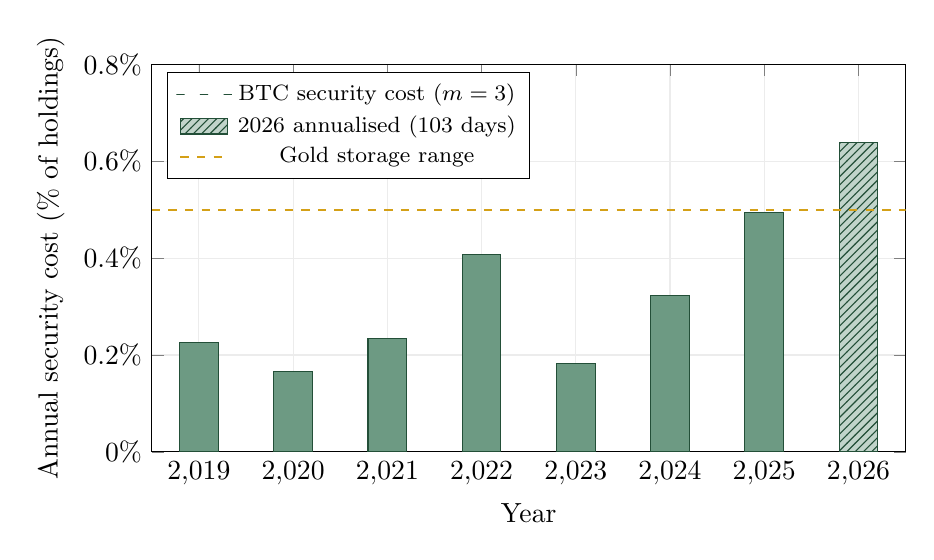
\begin{tikzpicture}
\begin{axis}[
  width=0.92\textwidth, height=6.5cm,
  xlabel={Year},
  ylabel={Annual security cost (\% of holdings)},
  ymin=0, ymax=0.8,
  xmin=2018.5, xmax=2026.5,
  xtick={2019,2020,2021,2022,2023,2024,2025,2026},
  yticklabel={\pgfmathprintnumber{\tick}\%},
  legend style={at={(0.02,0.98)},anchor=north west,font=\footnotesize},
  grid=major, grid style={gray!15},
]
\addplot[ybar, bar width=14pt, fill=accent!70, draw=accentdark] coordinates {
  (2019, \fpeval{\cXIX * 100})
  (2020, \fpeval{\cXX * 100})
  (2021, \fpeval{\cXXI * 100})
  (2022, \fpeval{\cXXII * 100})
  (2023, \fpeval{\cXXIII * 100})
  (2024, \fpeval{\cXXIV * 100})
  (2025, \fpeval{\cXXV * 100})
};
\addlegendentry{BTC security cost ($m = \UnderMult$)}

% 2026 bar: hatched only (no solid bar underneath)
\draw[fill=accent!30, draw=accentdark, postaction={pattern=north east lines, pattern color=accentdark}]
  ([xshift=-7pt]axis cs:2026, 0) rectangle ([xshift=7pt]axis cs:2026, \fpeval{\cXXVI * 100});
\addlegendimage{area legend, fill=accent!30, draw=accentdark, postaction={pattern=north east lines, pattern color=accentdark}}
\addlegendentry{2026 annualised (103 days)}

% Gold storage band
\addplot[goldcol, thick, dashed, domain=2018.5:2026.5, samples=2] {0.5};
\addplot[goldcol, thick, dotted, domain=2018.5:2026.5, samples=2] {1.5};
\addlegendentry{Gold storage range}
\end{axis}
\end{tikzpicture}
\captionof{figure}{Insurance-equivalent annual security cost for individual Bitcoin whales (green bars), compared to the institutional gold-storage cost range (gold dashed: 0.5--1.5\%/yr). The hatched 2026 bar is annualised from 103 days of data (\aXXVIytd{} attacks through April 13). At the current pace, the BTC security cost has entered the gold-storage range.}
\end{center}

% ── Chart: Attack rate per 100K whales ────────────────────────────────────
\begin{center}
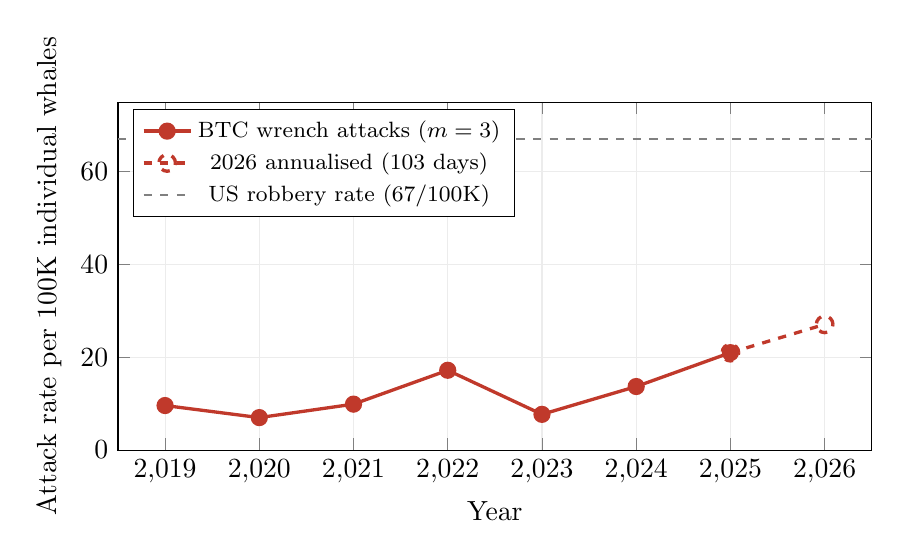
\begin{tikzpicture}
\begin{axis}[
  width=0.92\textwidth, height=6cm,
  xlabel={Year},
  ylabel={Attack rate per 100K individual whales},
  ymin=0, ymax=75,
  xmin=2018.5, xmax=2026.5,
  xtick={2019,2020,2021,2022,2023,2024,2025,2026},
  legend style={at={(0.02,0.98)},anchor=north west,font=\footnotesize},
  grid=major, grid style={gray!15},
]
\addplot[attackcol, very thick, mark=*, mark size=2.5] coordinates {
  (2019, \fpeval{round(\rhoXIX, 1)})
  (2020, \fpeval{round(\rhoXX, 1)})
  (2021, \fpeval{round(\rhoXXI, 1)})
  (2022, \fpeval{round(\rhoXXII, 1)})
  (2023, \fpeval{round(\rhoXXIII, 1)})
  (2024, \fpeval{round(\rhoXXIV, 1)})
  (2025, \fpeval{round(\rhoXXV, 1)})
};
\addlegendentry{BTC wrench attacks ($m = \UnderMult$)}

% 2026 annualized (open marker to indicate projection)
\addplot[attackcol, very thick, mark=o, mark size=3, dashed] coordinates {
  (2025, \fpeval{round(\rhoXXV, 1)})
  (2026, \fpeval{round(\rhoXXVI, 1)})
};
\addlegendentry{2026 annualised (103 days)}

% Reference: US robbery rate
\addplot[gray, thick, dashed, domain=2018.5:2026.5, samples=2] {67};
\addlegendentry{US robbery rate (67/100K)}
\end{axis}
\end{tikzpicture}
\captionof{figure}{Per-capita wrench-attack rate for individual Bitcoin whales (at $\UnderMult\times$ underreporting), compared to the US general robbery rate. The open circle for 2026 is annualised from 103 days of data. The 2026 pace (\fpeval{round(\rhoXXVI, 0)}/100K) represents a \fpeval{round((\rhoXXVI/\rhoXXV - 1) * 100, 0)}\% change relative to 2025.}
\end{center}

% ══════════════════════════════════════════════════════════════════════════
\section{Why the Trend Worsens}
\label{sec:trend}
% ══════════════════════════════════════════════════════════════════════════

\noindent The current security cost (\fpeval{round(\cXXVI * 100, 2)}\%/yr) understates the trajectory for several structural reasons:

\begin{enumerate}[leftmargin=1.5em]
  \item \textbf{Target identification is becoming easier.} Bitcoin is still held by far fewer people than jewelry, and typically more discreetly. Identifying a wrench attack target today requires blockchain analysis, social media intelligence, or insider knowledge --- skills less diffused than identifying a jewelry owner (visible watches, known stores, insured collections). But as adoption grows, Bitcoin wealth becomes statistically correlated with observable proxies (neighborhood, profession, social media). The targeting problem is converging toward the jewelry baseline.

  \item \textbf{Criminal skill sets are diffusing.} In 2014, a Bitcoin wrench attack required knowledge of wallets, private keys, and transfer mechanics. Today, a smartphone unlock and a Coinbase login suffice. The skill barrier is falling toward that of ordinary robbery.

  Obscurity-based defenses are a second layer of this same phenomenon --- and knowledge diffusion causes them to \textit{backfire}. Once an attacker learns what a decoy wallet is, they simply persist beyond the first transfer: the victim has complied, but the attacker has no way to know whether the disclosed wallet is the real one or a decoy. The rational response is to keep coercing. If the victim ``protects'' a UTXO via a two-path lock script --- path~A (clear key + $n$-block delay) vs.\ path~B (obscure redirect key) --- the victim complies using path~A and hopes the attacker is unaware of path~B, which can claw back the transfer during the delay window. An educated attacker who knows the scheme either coerces the victim to use the redirect key up front, or --- for good measure --- kills the victim after the coerced transfer to prevent them from redirecting it. In short, the efficacy of obscurity-based security is contingent on the premise that attackers are unable to acquire the same practical knowledge that defenders possess --- knowledge that, in Bitcoin's case, is open-source by design. As Kerckhoffs articulated in 1883: a system's security must not depend on the secrecy of its mechanism.\footnote{Kerckhoffs, A., ``La cryptographie militaire,'' \textit{Journal des sciences militaires}, 1883.} Obscurity violates this principle structurally.

  \item \textbf{The \$100K threshold is falling in BTC terms.} In 2014, \$100K required 314 BTC (early miners only). In 2025, it requires 1.1 BTC. The whale population is growing structurally as BTC appreciates, expanding the target set even without new adoption.

  \item \textbf{Attack CAGR exceeds whale CAGR.} Over 2019--2026, documented attacks grew at \fpeval{round(\gAtk * 100, 0)}\% per year while the individual whale population grew at \fpeval{round(\gWhale * 100, 0)}\%. The per-capita rate is increasing at a net \fpeval{round(\gNet * 100, 0)}\% annually.
\end{enumerate}

\noindent We are, in short, \textbf{early in the trend}. The current attack rate per whale (\fpeval{round(\rhoXXVI, 0)}/100K) is still well below mature crime categories like jewelry theft ($\sim$50--200/100K). As the targeting and skill barriers fall, convergence toward those rates is the natural trajectory.

% ══════════════════════════════════════════════════════════════════════════
\section{Forward-Looking Pricing}
% ══════════════════════════════════════════════════════════════════════════

\subsection{Why current cost understates the discount}

A significant component of Bitcoin's value is speculative: priced on the expectation of future adoption and appreciation. Speculative assets are particularly sensitive to trend changes in holding costs. The analogy is real estate: if a neighborhood has strong fundamentals (good schools, growing employment) but a visibly rising crime rate, housing prices drop \textit{before} the crime rate reaches high levels --- because buyers price in the trajectory, not just the current level. No single crime incident causes the repricing; it is the \textit{trend} that compounds into the discount.

Bitcoin exhibits the same structure. The market periodically attributes underperformance to rotating FUD cycles --- China mining bans, regulatory crackdowns, quantum computing fears --- each of which arrives, dominates a news cycle, and recedes. But the security tax does not recede. It compounds at \fpeval{round(\gNet * 100, 0)}\%/yr and is priced by no market. A rational long-term holder internalizes this cost whether or not it appears in any headline. To return to the analogy: the neighborhood's ``China ban'' scare comes and goes, but the rising break-in rate persists across all cycles. The persistent component is the one that reprices the asset.

We do not claim the security tax \textit{explains} Bitcoin's deviation from bullish models (stock-to-flow, etc.) --- too many confounds exist. We claim it is a \textbf{structurally compounding holding cost that is currently priced at zero}, and that any rational pricing model should subtract it. The attached present-value calculation quantifies how large that subtraction is.

\subsection{Estimating the growth rate $g$}

The net growth rate of the per-capita attack rate is the difference between the attack growth rate and the whale population growth rate. We estimate each as a CAGR over 2019--2026 (7 years), using the annualized 2026 attack count ($\fpeval{round(\aXXVIann, 0)}$):

\begin{align*}
  g_{\text{attack}} &= \left(\frac{a_{2026}^*}{a_{2019}}\right)^{1/7} - 1 = \left(\frac{\fpeval{round(\aXXVIann, 0)}}{\aXIX}\right)^{1/7} - 1 = \fpeval{round(\gAtk * 100, 1)}\%/\text{yr}\\[4pt]
  g_{\text{whale}} &= \left(\frac{W_{2026}}{W_{2019}}\right)^{1/7} - 1 = \left(\frac{\wXXVI}{\wXIX}\right)^{1/7} - 1 = \fpeval{round(\gWhale * 100, 1)}\%/\text{yr}\\[4pt]
  g_{\text{net}} &= \frac{1 + g_{\text{attack}}}{1 + g_{\text{whale}}} - 1 = \fpeval{round(\gNet * 100, 1)}\%/\text{yr}
\end{align*}

\noindent ($a_{2026}^*$ = annualized from \aXXVIytd{} attacks in \daysXXVI{} days.) The attack count is growing faster than the whale population, so the per-capita rate is rising at $\fpeval{round(\gNet * 100, 1)}$\%/yr. We exclude pre-2019 because whale populations below $\sim$250K make per-capita rates unreliable (see Section~\ref{sec:sensitivity}).

\subsection{Present value of expected security costs}

If the per-capita attack rate continues growing at $g = \fpeval{round(\gNet * 100, 1)}$\%/yr, the present value of security costs over a holding horizon $H$ is:

\begin{equation}
  D(t, H) = \sum_{k=0}^{H-1} \frac{c(t) \cdot (1 + g)^k}{(1 + r)^k} = c(t) \cdot \frac{q^H - 1}{q - 1}, \qquad q = \frac{1+g}{1+r}
  \label{eq:pv}
\end{equation}

\noindent The sum walks forward through each year of the holding period. In year $k$, the security cost has grown to $c(t) \cdot (1+g)^k$ --- because both the absolute attack count and the per-capita rate are increasing --- but that future cost is worth less today by the discount factor $(1+r)^{-k}$, where $r$ is the holder's required return. The ratio $q = (1+g)/(1+r)$ captures the race between cost growth and discounting:

\begin{itemize}[nosep,leftmargin=1.5em]
  \item When $g < r$: future costs grow, but discounting shrinks them faster. The series converges. Each additional year contributes less.
  \item When $g > r$: costs outrun discounting. Each additional year of holding contributes \textit{more} than the last, and the sum diverges for $H \to \infty$. This is the regime implied by the current data ($g \approx \fpeval{round(\gNet * 100, 0)}$\%, likely exceeding most real required returns).
\end{itemize}

\noindent $D(t,H)$ is the fraction of current holdings that a rational buyer should subtract from the asset's fundamental value to compensate for expected security costs over the next $H$ years. It is the present value of the stream of annual ``insurance premiums'' that no insurer offers.

\begin{center}
\small
\begin{tabular}{r r r}
\toprule
\textbf{Horizon} & $r = 10\%$ & $r = 15\%$ \\
\midrule
5 years  & \fpeval{round(\pvFiveTen * 100, 2)}\% & \fpeval{round(\pvFiveFif * 100, 2)}\% \\
10 years & \fpeval{round(\pvTenTen * 100, 2)}\% & \fpeval{round(\pvTenFif * 100, 2)}\% \\
\bottomrule
\end{tabular}
\end{center}

\noindent At a 10\% required return and 10-year horizon, the forward-looking discount is \fpeval{round(\pvTenTen * 100, 1)}\% --- roughly $\fpeval{round(\pvTenTen / \cXXVI, 0)}\times$ the current annual cost. This amplification occurs because the market must price in \textit{all} expected future security costs, not just this year's.

\medskip
\noindent\textbf{Caveat:} the \fpeval{round(\gNet * 100, 0)}\% net growth rate will not persist indefinitely --- either security solutions emerge (capping the cost) or adoption slows (reducing new whales). The finite-horizon formula is an upper bound under the assumption that the current trend continues. This is precisely the window in which intervention matters most.

% ══════════════════════════════════════════════════════════════════════════
\section{Comparison to Gold}
% ══════════════════════════════════════════════════════════════════════════

Gold is the natural comparator: a portable store of value that faced the same physical vulnerability problem over centuries.

\begin{center}
\small
\begin{tabular}{l r r}
\toprule
& \textbf{Gold (vaulted)} & \textbf{BTC (self-custody)} \\
\midrule
Annual holding cost & 0.5--1.5\%\footnote{APMEX/Citadel: 0.45--0.55\%; Hard Assets Alliance: 0.50--0.70\%; Perth Mint (allocated): $\sim$1.5\%.} & \fpeval{round(\cXXVI * 100, 2)}\% (and rising) \\
Insurance available & Yes (mature market) & No \\
Loss per event & Partial ($\sim$30\%) & Total (100\%) \\
Cost trend & Stable & Worsening (+\fpeval{round(\gNet * 100, 0)}\%/yr) \\
Security infrastructure & Vaults, Brinks, Fort Knox & ``Don't tell anyone'' \\
\bottomrule
\end{tabular}
\end{center}

\noindent Gold's explicit storage/insurance costs are \textit{known, stable, and priced}. Bitcoin's implicit security costs are \textit{uncertain, growing, and unpriced} --- exactly the conditions under which risk-averse capital rotates away.

The concurrent gold surge (from \$1,393/oz in 2019 to \$3,435/oz in 2025, +147\%) is consistent with this rotation. Capital that might otherwise flow into BTC as a store of value flows instead into an asset whose security costs are solved, explicit, and declining in real terms.

% ══════════════════════════════════════════════════════════════════════════
\section{Robustness}
\label{sec:sensitivity}
% ══════════════════════════════════════════════════════════════════════════

\subsection{Sensitivity to underreporting multiplier}

\begin{center}
\small
\begin{tabular}{r r r r}
\toprule
\textbf{Multiplier} $m$ & \textbf{2026 rate/100K} & \textbf{2026 cost} & \textbf{10-yr PV ($r$=10\%)} \\
\midrule
$1\times$ (reported only)
  & \fpeval{round(\aXXVIann * 1 * 100 / \wXXVI, 1)}
  & \fpeval{round(\cCurOneX * 100, 3)}\%
  & \fpeval{round(\cCurOneX * (exp(10*ln(\qTen)) - 1) / (\qTen - 1) * 100, 2)}\% \\
\rowcolor{accentlight}
$3\times$ (Lopp estimate)
  & \fpeval{round(\rhoXXVI, 1)}
  & \fpeval{round(\cXXVI * 100, 3)}\%
  & \fpeval{round(\pvTenTen * 100, 2)}\% \\
$10\times$ (aggressive)
  & \fpeval{round(\aXXVIann * 10 * 100 / \wXXVI, 1)}
  & \fpeval{round(\cCurTenX * 100, 3)}\%
  & \fpeval{round(\cCurTenX * (exp(10*ln(\qTen)) - 1) / (\qTen - 1) * 100, 2)}\% \\
\bottomrule
\end{tabular}
\end{center}

{\footnotesize The underreporting multiplier scales both the annual cost and the PV linearly. Even at $1\times$ (reported attacks only), the 10-year forward-looking discount is non-trivial.}

\medskip
\noindent\textbf{Why $m = 3$ is conservative.} Jewelry theft provides a floor for calibrating underreporting, because it is the closest analog (portable, high-value, personally held) with established victimization survey data. The NCVS--UCR gap for property crime implies that only $\sim$30--33\% of property crimes are reported to police.\footnote{BJS, \textit{Criminal Victimization, 2022}; see also Skogan, W.G., ``Dimensions of the Dark Figure of Unreported Crime,'' \textit{Crime \& Delinquency} 23(1), 1977.} Reporting rates vary sharply with insurance status:

\begin{center}
\small
\begin{tabular}{l r r}
\toprule
\textbf{Jewelry victim profile} & \textbf{Est.\ reporting rate} & \textbf{Implied $m$} \\
\midrule
Insured, declared & 50--65\% & $\sim$1.5--2$\times$ \\
Uninsured, nothing to hide & 25--35\% & $\sim$3--4$\times$ \\
Undeclared / off-book holdings & 5--15\% & $\sim$7--20$\times$ \\
\bottomrule
\end{tabular}
\end{center}

{\footnotesize Insurance is the dominant driver of reporting: a police reference number is required to file a claim.\footnote{BJS, \textit{Reporting Crimes to the Police} (Harlow, 1985): for losses $\geq$\$250, ``economic incentives (to collect insurance or recover property) dominated.''} Over 60\% of Americans carry no jewelry insurance.\footnote{ValuePenguin, ``More Than 6 in 10 Say Their Jewelry Is Uninsured,'' 2023.} For undeclared assets, reporting the theft means documenting holdings the victim never disclosed --- creating exposure for tax evasion, customs violations, or unreported inheritance. The FINRA Foundation finds that only $\sim$15\% of financial fraud victims report, with shame and self-blame as the primary barriers.\footnote{FINRA Foundation, \textit{Blame and Shame in the Context of Financial Fraud}, 2021.}}

\smallskip
\noindent Bitcoin wrench attacks compound every factor that suppresses jewelry reporting, then add more:

\begin{itemize}[nosep,leftmargin=1.5em]
  \item \textbf{No insurance exists} --- the single largest driver of property-crime reporting is entirely absent.
  \item \textbf{Recovery rate is zero} --- transferred BTC is irrecoverable; there is no property to recover.
  \item \textbf{Cultural norm is non-disclosure} --- the community's own security advice (``don't tell anyone you own Bitcoin'') primes victims against reporting.
  \item \textbf{Undeclared holdings are prevalent} --- BTC held for tax optimization, sanction avoidance, or simply outside the regulated financial system creates an active \textit{disincentive} to involve authorities. Reporting the attack means documenting assets the victim never disclosed.
  \item \textbf{Victim-blaming compounds shame} --- ``you should have used cold storage'' / ``you shouldn't have told anyone'' mirrors the shame dynamic that suppresses fraud reporting to $\sim$15\%.
\end{itemize}

\noindent If \textit{insured} jewelry --- the most-reported category of portable-valuables theft --- already implies $m \approx 1.5$--$2$, and \textit{uninsured off-book} jewelry reaches $m \approx 7$--$20$, then Bitcoin --- which shares every underreporting factor with jewelry and adds several more --- should sit well above the jewelry floor. The $m = 3$ baseline is better understood as the \textit{lower bound of the jewelry analog}, not a Bitcoin-specific estimate. A range of $m = 5$--$10$ is defensible; the $m = 10$ row in the table above may be closer to ground truth than the highlighted baseline.

\subsection{Sensitivity to severity multiplier}

\begin{center}
\small
\begin{tabular}{r l r r}
\toprule
$\sigma$ & \textbf{Interpretation} & \textbf{2026 cost} & \textbf{10-yr PV ($r$=10\%)} \\
\midrule
3 & Total loss only; no uninsured premium
  & \fpeval{round(\cXXVI / \SevMult * 3 * 100, 3)}\%
  & \fpeval{round(\pvTenTen / \SevMult * 3 * 100, 2)}\% \\
\rowcolor{accentlight}
6 & Baseline (total loss $\times$ uninsured)
  & \fpeval{round(\cXXVI * 100, 3)}\%
  & \fpeval{round(\pvTenTen * 100, 2)}\% \\
10 & Including violence/trauma premium
  & \fpeval{round(\cXXVI / \SevMult * 10 * 100, 3)}\%
  & \fpeval{round(\pvTenTen / \SevMult * 10 * 100, 2)}\% \\
15 & Full irrecoverability + behavioral premium
  & \fpeval{round(\cXXVI / \SevMult * 15 * 100, 3)}\%
  & \fpeval{round(\pvTenTen / \SevMult * 15 * 100, 2)}\% \\
\bottomrule
\end{tabular}
\end{center}

{\footnotesize At $\sigma = 15$ (defensible if behavioral/psychological costs are included), the 10-year discount reaches \fpeval{round(\pvTenTen / \SevMult * 15 * 100, 1)}\%.}

\subsection{Sensitivity to whale population}

The whale population estimates are the least certain input. We show the 2026 security cost at three population levels:

\begin{center}
\small
\begin{tabular}{r r r r}
\toprule
\textbf{Whale pop.\ (2026)} & \textbf{Rate/100K} & \textbf{Ann.\ cost} & \textbf{10-yr PV ($r$=10\%)} \\
\midrule
500K (conservative) & \fpeval{round(\aXXVIann * \UnderMult * 100 / 500, 1)} & \fpeval{round(\aXXVIann * \UnderMult * 100 / 500 * \kappa * 100, 3)}\%
  & \fpeval{round(\aXXVIann * \UnderMult * 100 / 500 * \kappa * (exp(10*ln(\qTen)) - 1) / (\qTen - 1) * 100, 2)}\% \\
\rowcolor{accentlight}
1\,100K (baseline) & \fpeval{round(\rhoXXVI, 1)} & \fpeval{round(\cXXVI * 100, 3)}\%
  & \fpeval{round(\pvTenTen * 100, 2)}\% \\
2\,000K (generous) & \fpeval{round(\aXXVIann * \UnderMult * 100 / 2000, 1)} & \fpeval{round(\aXXVIann * \UnderMult * 100 / 2000 * \kappa * 100, 3)}\%
  & \fpeval{round(\aXXVIann * \UnderMult * 100 / 2000 * \kappa * (exp(10*ln(\qTen)) - 1) / (\qTen - 1) * 100, 2)}\% \\
\bottomrule
\end{tabular}
\end{center}

{\footnotesize Even with 2M whales (generous upper bound), the 10-year discount remains material.}

% ══════════════════════════════════════════════════════════════════════════
\section{Limitations}
% ══════════════════════════════════════════════════════════════════════════

\begin{enumerate}[nosep,leftmargin=1.5em]
  \item \textbf{Whale population estimates are rough.} On-chain data conflates addresses with individuals, and institutional vs.\ personal holdings are not cleanly separable. We mitigate this with sensitivity analysis (Section~\ref{sec:sensitivity}).
  \item \textbf{The severity multiplier is a judgment call.} The $\sigma = 6$ baseline is conservative and grounded (total-loss ratio $\times$ uninsured premium), but the true behavioral discount could be higher or lower.
  \item \textbf{Underreporting is uncertain.} Lopp estimates 2--3$\times$; law enforcement suggests it could be higher. The model is linear in $m$.
  \item \textbf{The insurance analogy is approximate.} Jewelry insurance pricing reflects a mature market with actuarial data, loss adjusters, and reinsurance. Applying the same per-unit-of-crime pricing to Bitcoin is a first-order transfer, not an exact calibration.
  \item \textbf{Growth rates will not persist.} The \fpeval{round(\gNet * 100, 0)}\% net growth rate of per-capita attacks implies convergence toward mature crime rates within a decade. The model assumes constant growth over the horizon; reality will involve plateaus and discontinuities.
  \item \textbf{No behavioral/media amplification factor.} The model prices actuarial risk only. The ``SF Union Square effect'' --- where anti-crime measures and media coverage suppress demand far beyond the actuarial loss --- is real but not quantified here. The insurance-based estimate is therefore a \textit{lower bound}.
\end{enumerate}

% ══════════════════════════════════════════════════════════════════════════
\section{Testable Predictions}
% ══════════════════════════════════════════════════════════════════════════

\begin{enumerate}[leftmargin=1.5em]
  \item \textbf{Insurance market emergence.} If the security cost estimate is correct, an insurance market for self-custody BTC should emerge with premiums in the 0.5--2\% range. Lloyd's of London or specialty crypto insurers are the likely first movers.
  \item \textbf{Luxury-goods crime correlation.} The geographic distribution of wrench attacks (per Lopp's tracker) should correlate with luxury-goods crime indices. France's outsized share of attacks should correlate with France's jewelry/watch robbery rates.
  \item \textbf{Whale migration to custodial solutions.} As the security cost rises, the fraction of whale-held BTC in self-custody should \textit{decrease} in favor of institutional custody and ETFs, despite the community's philosophical preference for self-sovereignty.
  \item \textbf{The 2026 trajectory --- tracking the model.} The 2025-based projection implied $\sim$90 attacks for 2026 on a trend-line extrapolation. As of April 13, 2026, \aXXVIytd{} attacks have been documented in 103 days --- an annualised pace of $\fpeval{round(\aXXVIann, 0)}$, already above the full-year 2025 total and within $\fpeval{round(abs(\aXXVIann / 90 - 1) * 100, 0)}\%$ of the extrapolation. At that pace, the 2026 annual security cost reaches \fpeval{round(\cXXVI * 100, 3)}\%, firmly inside the gold-storage range. The acceleration remains concentrated in France (20 of \aXXVIytd{} YTD attacks), where data breaches have created target-rich conditions.
  \item \textbf{Great Wall adoption should suppress the cost trajectory.} If coercion-resistant custody reaches meaningful share among individual whales, the effective severity multiplier should decline (both loss probability and loss magnitude fall), providing a natural experiment.
\end{enumerate}

% ══════════════════════════════════════════════════════════════════════════
\section{What Great Wall Does About It}
% ══════════════════════════════════════════════════════════════════════════

The security tax reframes Great Wall's value proposition in concrete, defensible terms:

\begin{center}
\large\bfseries\itshape
Great Wall eliminates an implicit annual holding cost that already sits inside the gold-storage range --- without requiring obscurity, custodial trust, or a self-sovereignty compromise.
\end{center}

\noindent Great Wall is a free-software self-custody Bitcoin wallet, dual-licensed under MIT or Apache-2.0, in which the seed lives only in the user's memory. The authentication secret is encoded onto a user-specific perturbation of the Burning Ship fractal; recall is spatial-visual, and --- as elaborated below --- the holder \emph{cannot articulate} the secret in a form an attacker could transcribe. The entry point is gated by a calibrated Argon2 derivation whose target duration is benchmarked against Jameson Lopp's published wrench-attack corpus, so that no published custody window would have sufficed to extract the secret.

Scale matters for the argument. At the current annualised cost of \fpeval{round(\cXXVI * 100, 2)}\%, a whale population of $\sim$1.1M individuals, and an average of $\sim$\$300K per whale in BTC, the aggregate annual security tax is approximately:

\begin{equation*}
  \fpeval{round(\cXXVI * 100, 2)}\% \times 1{,}100{,}000 \times \$300{,}000 = \$\fpeval{round(\cXXVI * 1100000 * 300000 / 1000000, 0)}\text{M/year}
\end{equation*}

\noindent Over a 10-year horizon with the forward-looking multiplier, the present value of the security tax across the whale population is \fpeval{round(\pvTenTen * 100, 1)}\% of \$\fpeval{round(\WhaleAUMbn, 0)}B $\approx$ \$\fpeval{round(\TenYrTAMbn, 1)}B. That figure is value being destroyed across the entire Bitcoin ecosystem, not a revenue projection. The engineering path through which Great Wall eliminates it --- fractal encoder, time-lock-puzzle library, spaced-repetition training vault, Lightning marketplace for outsourced solving, dead-man's-switch inheritance protocol, and the unified desktop wallet that integrates them --- is the subject of the sections that follow.

\subsection{The protocol is application-agnostic}

Great Wall's time-lock layer enforces a cryptographic delay on any secret --- Bitcoin keys being the first and most natural use case, but any application requiring a verifiable off-chain delay fits the same primitive. The protocol is open and runs entirely locally; only the \emph{serial computation} that imposes the time-lock is outsourced, to an anonymous Lightning-Network marketplace whose role is to sell compute, not custody.

\subsubsection{Time-lock mechanics}

Great Wall's time-lock is built on \textit{repeated modular squaring}, the construction proposed by Rivest, Shamir, and Wagner (1996)\footnote{Rivest, R.L., Shamir, A. \& Wagner, D.A., ``Time-Lock Puzzles and Timed-Release Crypto,'' MIT/LCS/TR-684, 1996.} and refined by modern Verifiable Delay Functions.\footnote{Boneh, D. et al., ``Verifiable Delay Functions,'' \textit{CRYPTO 2018}, LNCS 10991; Wesolowski, B., ``Efficient Verifiable Delay Functions,'' \textit{EUROCRYPT 2019}, LNCS 11478; Pietrzak, K., ``Simple Verifiable Delay Functions,'' \textit{ITCS 2019}, LIPIcs 124.} The setup:

\begin{itemize}[nosep,leftmargin=1.5em]
  \item Choose an RSA modulus $n = pq$ of $b$ bits (e.g.\ $b = 2048$).
  \item To lock for a target delay $d$: set $T = d \times s_{\max}$, where $s_{\max}$ is the squarings-per-second of the fastest plausible hardware.
  \item Unlocking requires computing $x^{2^T} \bmod n$ --- exactly $T$ sequential squarings.
  \item \textbf{Critical property:} without the factorization of $n$, this computation \textit{cannot be parallelized}. Ten thousand cores offer zero speedup. Only single-pipeline sequential throughput matters.
\end{itemize}

\noindent The three variables are the modulus size $b$, the iteration count $T$, and the hardware squaring rate $s(b, H)$ for hardware class $H$. The squaring rate scales as $s(b,H) \approx C(H) / b^\alpha$, where $\alpha \approx 2$ (Montgomery multiplication\footnote{Montgomery, P.L., ``Modular Multiplication Without Trial Division,'' \textit{Math.\ of Computation} 44(170), 1985.}) and $C(H)$ captures clock speed, IPC, and algorithmic tuning.

The \textbf{convenience ratio} $R = C(H_{\max}) / C(H_{\text{user}})$ determines how many multiples of the minimum delay a given client experiences. Crucially, $R$ is \textbf{independent of $b$}: the modulus cancels in the ratio. Choosing a larger modulus makes every tier proportionally slower but does not change the relative speed spread. The modulus should be chosen for cryptographic soundness (2048+ bits), not as a pricing lever.

Because the computation is inherently sequential, the speed spread across \textit{all available hardware} is compressed to single-pipeline performance differences --- roughly 10--30$\times$ from consumer laptop to hypothetical ASIC. This is simultaneously a \textbf{feature} (the attacker's advantage over any client is bounded by this narrow band) and a \textbf{constraint} (limited room for tier differentiation).

The guaranteed delay is hardware-contingent: $d = T / s_{\max}$ holds as long as $s_{\max}$ reflects the state of the art. In practice this is bounded: Moore's law yields $\sim$1.1--1.2$\times$/yr for single-thread performance, and the user re-calibrates $T$ at each vault refresh cycle ($\sim$weekly). A VDF construction adds efficient verifiability --- the solver returns a short proof of correct computation, removing the need to trust the solver.

\medskip
\noindent\textbf{Why weekly: the TKBA refresh cycle.} Great Wall's coercion resistance rests on \href{https://en.wikipedia.org/wiki/Tacit_knowledge}{\textit{Tacit Knowledge-Based Authentication}} (TKBA) --- authentication by navigating to a randomly generated identifiable location in a fractal landscape. Because all reference points in a fractal are self-similar, abstract, and jagged, the location is nearly impossible to verbally describe or sketch --- even under duress. The holder recognises and navigates to their point, but cannot \textit{communicate} it --- Polanyi's ``we can know more than we can tell.''\footnote{Polanyi, M., \textit{The Tacit Dimension}, Routledge \& Kegan Paul, 1966.} This spatial memory is subject to \textit{catastrophic forgetting} if not periodically rehearsed.\footnote{Ebbinghaus, H., \textit{{\"U}ber das Ged{\"a}chtnis}, 1885; Murre, J.M.J. \& Dros, J., ``Replication and Analysis of Ebbinghaus' Forgetting Curve,'' \textit{PLOS ONE} 10(7), 2015.} The vault refresh cycle ($\sim$weekly) is therefore not arbitrary: it is the cadence at which the holder must \textit{revisit} their fractal location to maintain reliable recall. This same cycle conveniently re-calibrates $T$ against the current computational state of the art and generates a steady stream of puzzles for the anonymity set.

\subsubsection{Transport: Lightning Network + Tor}

The marketplace runs natively over the \textbf{Lightning Network}. Puzzles, solutions, and payments all flow over the same LN channels, using onion-routed payments. Combined with Tor (already supported by LN wallets such as Phoenix and Zeus), the puzzle submission is unlinkable to the submitter. This solves three problems simultaneously:

\begin{itemize}[nosep,leftmargin=1.5em]
  \item \textbf{Payment privacy.} Per-puzzle fees are micropayments --- exactly what LN is designed for. No on-chain footprint per transaction.
  \item \textbf{Puzzle privacy.} The puzzle and its solution travel over the same onion-routed channel as the payment. No separate transport protocol needed.
  \item \textbf{Infrastructure perk.} Both clients and solvers become well-connected LN nodes. If the marketplace achieves scale, its channel graph becomes significant LN routing infrastructure. Participants gain high-connectivity wallets useful for \textit{all} LN payments, not just GW --- creating stickiness beyond the anonymity set.
\end{itemize}

\subsubsection{A note on the marketplace posture}

Whatever fees the marketplace ultimately charges must be \emph{value-blind}: holders do not want to disclose how much (or what) their time-lock protects, so any AUM-based or value-proportional scheme would leak the very information the scheme is designed to protect. A flat per-puzzle fee is the only posture consistent with the privacy property. This document does not propose a fee schedule; it notes only that the privacy constraint rules out any fee that is a function of the protected value, and that the anonymity set itself --- the pool of concurrent puzzles among which any individual puzzle is indistinguishable --- is the core property the marketplace has to preserve.

\subsubsection{Inheritance as a dead-man's switch}
\label{sec:inheritance}

The same time-lock infrastructure underwrites a trustless inheritance protocol. Its role in this document is technical --- it shows that one building block, the RSW time-lock, is doing double duty for coercion resistance and for post-mortem transfer --- rather than commercial.

\medskip
\noindent\textbf{Setup.} A testator (Ted) holds BTC across LN channels with GW marketplace nodes and wishes to distribute portions $p_1, p_2, \ldots$ to heirs Henry, Harry, etc.

\begin{enumerate}[nosep,leftmargin=1.5em]
  \item Ted creates an HTLC (Hash Time-Locked Contract) in his GW channel: ``Pay $p_1$ to Henry's key if the preimage of hash $H$ is revealed.''
  \item A time-lock puzzle, when solved, reveals the preimage.
  \item Ted broadcasts the puzzle to Henry via LN (onion-routed, private).
  \item \textbf{Rotation:} Before the puzzle is solved, Ted cancels the old HTLC and creates a new one with a fresh hash --- both are channel state updates, \textit{entirely off-chain}. The old puzzle, even if eventually solved, reveals a preimage for an HTLC that no longer exists.
  \item While Ted is alive and competent, he rotates periodically ($\sim$weekly). Each rotation invalidates the previous puzzle and issues a new one.
  \item \textbf{Trigger:} When Ted dies or becomes incapacitated, rotation stops. The current puzzle runs to completion. Henry solves it, reveals the preimage, and claims the HTLC.
\end{enumerate}

\noindent\textbf{Key properties:}

\begin{itemize}[nosep,leftmargin=1.5em]
  \item \textbf{No trusted third party.} No lawyer, no custodian, no multisig co-signer. The cryptographic time-lock \textit{is} the dead man's switch.
  \item \textbf{No on-chain footprint during Ted's lifetime.} HTLC creation, cancellation, and rotation are channel state updates --- off-chain. Ted's BTC stays in existing LN channels; rotation moves balances between channels via circular LN payments (also off-chain). The only on-chain transaction occurs when an heir force-closes a channel to claim inheritance --- after Ted's death, when privacy no longer matters.
  \item \textbf{Proportional distribution.} Different heirs receive different portions, each with its own HTLC and puzzle stream.
  \item \textbf{Automatic trigger.} No ``death oracle'' or certificate needed. Cessation of rotation \textit{is} the trigger.
\end{itemize}

\noindent\textbf{Anonymity-set contribution.} A testator with three heirs rotating weekly issues $3 \times 52 = 156$ puzzles per year. These outstanding (unsolved) puzzles pad the anonymity set for anti-coercion users --- more concurrent puzzles in the pool means better privacy for everyone --- but are not themselves solved until rotation stops. Inheritance and anti-coercion are therefore mutually reinforcing at the protocol level: each increases the other's anonymity-set depth without requiring coordination.

% ══════════════════════════════════════════════════════════════════════════
\section{Why This Is Bitcoin-Ecosystem Infrastructure}
% ══════════════════════════════════════════════════════════════════════════

The argument of this document is simple: the Bitcoin community has a measurable, compounding physical-security cost that it currently prices at zero, that its consensus defence (obscurity) fails to address and indeed contradicts in its own terms, and that a purely cryptographic alternative exists and is implementable from existing primitives. The Great Wall deliverables --- fractal encoder, time-lock-puzzle library, spaced-repetition training vault, anonymous Lightning marketplace for outsourced solving, dead-man's-switch inheritance protocol, and a unified desktop wallet integrating the six libraries --- are the engineering path from the pricing argument to a working system.

The project's posture is that of ecosystem infrastructure:

\begin{enumerate}[nosep,leftmargin=1.5em]
  \item \textbf{Every wrench attack is a news cycle reinforcing that self-custody is unsafe, and every ``don't tell anyone you own Bitcoin'' is a brake on adoption.} The security tax quantified above --- \$\fpeval{round(\AnnualTAMbn * 1000, 0)}M per year and growing at \fpeval{round(\gNet * 100, 0)}\%/yr --- is value being destroyed across the entire Bitcoin ecosystem. A working TKBA wallet eliminates it.
  \item \textbf{Standard Bitcoin primitives only; no soft fork ask.} Taproot outputs, MuSig2 aggregation, standard Lightning commitment/revocation, BIP39/BIP32 derivation, secp256k1. The time-lock lives one layer above the script, wrapping key material rather than adding a new opcode.
  \item \textbf{Reusable building blocks.} The RSW time-lock library, the anonymous LN marketplace client, and the dead-man's-switch channel pattern are independently useful for any other Bitcoin project that needs long-horizon conditional spending without covenants.
  \item \textbf{Purely free software.} All seven repositories are dual-licensed MIT or Apache-2.0. There is no equity, no token, no pre-sale, no valuation overlay. A prior commercially-structured attempt at the same core idea was wound down; the current effort is a clean-slate restart into the grant-funded open-source posture described here.
\end{enumerate}

\noindent The return is primarily an \emph{externality}: a healthier Bitcoin ecosystem benefits every participant. This document makes the analytical case for why that software is worth producing; the engineering time required to produce it is the subject of the Great Wall repositories referenced in the footer.

\vspace{16pt}
\noindent{\small\itshape\color{graytext}
The insurance-based framework provides a lower bound on the security cost (actuarial only, no behavioural amplification). All values are computed live by \LaTeX{} from the parameters in the preamble; changing any assumption recomputes the entire analysis.\\[4pt]
Great Wall umbrella repository: \url{https://github.com/Yuri-SVB/Great-Wallet}.\\[2pt]
Attack data: \url{https://github.com/jlopp/physical-bitcoin-attacks} (refreshed 22 April 2026; 2026 figures above reflect the Jan--Apr~13 window in that tracker).
}

\end{document}
